\section{Kotači}
Kako je navedeno u prethodnom poglavlju kotači se sastoje od više komponenti. Te komponente su mreža (\emph{eng. Mesh}), transformacija, te mrežni prevoditelj (\emph{eng. Mesh Renderer}) koji dopušta korisniku da vidi konačni element. Ono što se koristi za kretanje modela je kolni sudarač. Mreža se može vidjeti na slici \ref{fig:kotaci} desno, a sudarač na slici \ref{fig:kotaci} lijevo. \par
Isto tako veoma bitna stvar je povećati masu modela, inače će početi nekontrolirano rotirati na sceni, kao da je upalo u crnu rupu. Vrijednost u konačnici definira kojom silom će gravitacija privlačiti model, odnosno definiramo brzinu. Što je masa veća sporiji je igrajući objekt i obrnuto.

\begin{figure}[h]
	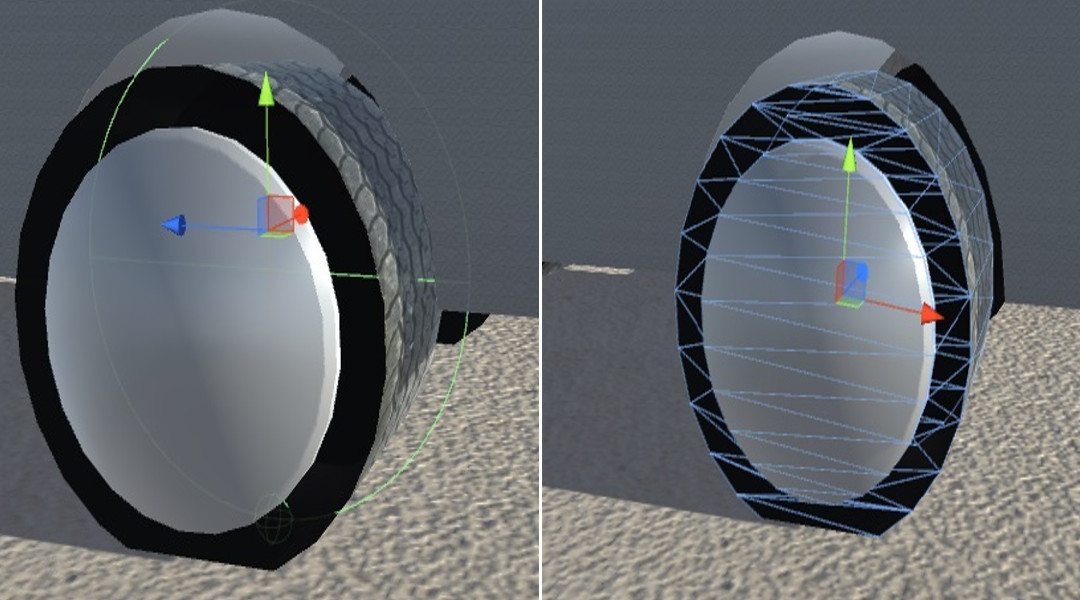
\includegraphics[width=12.5cm, height=6.5cm]{wheels.jpg}
	\centering
	\caption{Kotači modela}
	\label{fig:kotaci}
\end{figure}

\subsection{Rotiranje kotača}
Prilikom vožnje automobila za bolju simulaciju potrebno je okretati i kola. Za isprogramirati ovu naizgled jednostavnu radnju više stvari treba unaprijed biti dobro definirano, inače se stvar komplicira. Ukoliko je igrajući objekt loše definiran i pivoti nisu dobro postavljeni na kotačima, zbog mehanike koju unity koristi objekti rotiraju krivo ili treba koristit naprednije metode koje povećavaju broj linija koda i stvaraju dodatne probleme. Rotacija kotača bi trebala biti oko njegove osi, te se zato mora postaviti pivot u sredinu kotača. Ovo se obavlja tijekom izrade samog modela, te treba paziti na to prije unosa u unity. Ako se pivot nije centrirao prilikom izrade, onda se treba obavljati popravljanje. Koraci za popravljanje:
\begin{enumerate}
	\item Pronaći objekt (kotač) unutar hijerarhije
	\item Napraviti novi prazni objekt na istoj razini kao i kotač
	\item Kotač ubaciti u prazni objekt
\end{enumerate}
Sada za okretanje kotača se koristi novi prazni objekt jer je njegov pivot centriran. Ovakav pristup je jako učestal zbog dizajnera koji ne paze na pivote unutar svojih modela. Skripta za okretanje kola se može vidjeti u ispisu \ref{okretanjeKola}:
\begin{lstlisting}[caption={Skripta za okretanje kola}, label=okretanjeKola]
for (int i = 0; i < 4; i++) 
			this.tirePivots[i].transform.Rotate(
			    Vector3.forward, 
			    this.speed * move * Time.deltaTime
			);	
\end{lstlisting}
\subsection{Problemi u zavojima}
Prilikom vožnje vozila dodavanjem samo kolnih sudarača ne bismo dobili potpunu imitaciju pravog vozila. Jedan od problema koji se javlja je preokretanje u zavojima. Ova pojava je sasvim opravdana i nije nikakva greška programa. Što se ustvari događa? Kada vozilo uđe u zavoj i započme skretanje, na njega djeluje centrifugalna sila, podigne se prednji kotač sa tla i kako ne postoji protusila preokrene se. \par
Za ovaj slučaj postoji više rješenja, a onaj koji se koristi u igrici je sljedeći. Pri skretanju se provjeri koji kotač se podiže od tla i na njega se primjeni sila koja djeluje u smjeru gravitacije. Na ovaj način se smanji utjecaj centrifugalne sile, te samim time teže preokrenuti vozilo.
